\documentclass[runningheads]{llncs}
\usepackage[T1]{fontenc}
\usepackage{graphicx}
\usepackage{algorithm}
\usepackage{algpseudocode}
\usepackage{amsmath}
\usepackage{tikz}
\usetikzlibrary{matrix, positioning, arrows.meta, backgrounds}
\usepackage{booktabs}
\usepackage{svg}
\usepackage{url}
\usepackage{subcaption}
\def\UrlBreaks{\do\/\do-\do.\do=\do_\do?\do\&}
\input{mymacros}

%%%%%%%%%%%%%%%%%%%%%%%%%%%%%%%%%%%%%%%%%%%%%%%%%%%%
\begin{document}
\title{GNN-Guided Graph Partitioning for Spatial CGRA Mapping}
%
\author{Deniz Lopes Gunes\inst{1}\orcidID{0000-1111-2222-3333} \and
Henrique Teixeira\inst{1}\orcidID{1111-2222-3333-4444} \and
Guilherme Oliveira\inst{1}\orcidID{2222-3333-4444-5555} \and
Nuno Paulino\inst{1}\orcidID{3333-4444-5555-6666}}
%
\authorrunning{D. L. Gunes et al.}
% First names are abbreviated in the running head.
% If there are more than two authors, 'et al.' is used.
%
\institute{INESC TEC, Porto, Portugal\\
\email{\{deniz.l.gunes,henrique.santos.teixeira,\\guilherme.oliveira,nuno.m.paulino\}@inesctec.pt}}
%
\maketitle              % typeset the header of the contribution

%%%%%%%%%%%%%%%%%%%%%%%%%%%%%%%%%%%%%%%%%%%%%%%%%%%
\begin{abstract}
Mapping Data-Flow Graphs (DFGs) onto Coarse-Grained Reconfigurable Arrays (CGRAs) requires partitioning the graph into resource-feasible subgraphs when the DFG exceeds CGRA capacity. The quality of this partitioning directly impacts execution efficiency: each cut edge incurs communication overhead due to data transfer. Exact methods such as exhaustive SAT-based min-K partitioning yield optimal cuts but scale poorly; greedy heuristics are fast but produce poor partitions and frequently fail on wide, parallel graphs.
%
This paper proposes a GNN-guided partitioning flow that learns optimal 
%partition structure 
graph partitions, by learning
from SAT-generated ground truth. 
%A GNN classifier 
The GNN predicts per-node partition assignments, which seed a topology-aware partitioner that convexifies dependency ordering and repairs capacity violations to guarantee feasibility. On a synthetically generated 4×4 homogeneous CGRA dataset (1650 synthetic graphs; 150 held-out for evaluation), the GNN-guided partitioner reduces edge cuts by $\sim$1.07 per graph relative to the unguided baseline ($\approx$33\% relative reduction, roughly halving the gap to the SAT optimum), maps 98\% of graphs versus 15\% for greedy list scheduling, and runs at $\sim$0.25 s per graph; approximately 50× faster than the exact SAT solver.
\keywords{Coarse-Grained Reconfigurable Arrays \and Graph Partitioning \and Graph Neural Networks \and Spatial Mapping \and Data-Flow Graphs \and SAT-Based Mapping}
\end{abstract}

%%%%%%%%%%%%%%%%%%%%%%%%%%%%%%%%%%%%%%%%%%%%%%%%%%%%%%%%%%%%%%%%%%%%%%%%%%%%%%%%%%%%%%%
\section{Introduction}
% Motivation:
% - CGRA mapping scalability
% - Large DFGs require partitioning
% - Partition quality affects memory movement and mapping complexity
%
% Main idea:
% - Learn partition guidance from exhaustive search
%
% Contributions:
% - Synthetic dataset generation
% - SAT-min-K ground-truth generation
% - GNN-guided greedy partitioning
% - Experimental evaluation on synthetic graphs

Coarse-Grained Reconfigurable Arrays (CGRAs) have been a topic of hardware architecture research for three decades, and despite extant limitations, they are the target of newfound interest due to emergence of Edge AI applications, such as Small Language Models or multi-modal transformers. The bulk of the processing in these workloads is based on matrix multiplication, and thus the spatial parallelism of CGRAs promises processing benefits, especially when considering embedded and edge scenarios which can also benefit from the open-source RISC-V ecosystem for accelerated integration and cost-free IP use.

%Coarse-Grained Reconfigurable %Arrays 
%Arrays (CGRAs) have become more relevant in this age of artificial intelligence (AI), Large Language Models (LLMs) and machine learning. By leveraging the flexibility of programmable processors with the efficiency of hardware accelerators, these architectures are increasingly relevant for accelerating compute-intensive workflows, targeting domains such as signal processing and neural network inference. 

However, mapping computation, which is typically in the form of Data-Flow Graphs (DFGs), onto CGRAs remains an NP-Hard problem. 
%Due to limited spatial resources and routing constraints, mapping a DFG onto a CGRA can quickly become 
It is a placement and routing problem which becomes
%The problem becomes 
computationally very expensive, as the size of the CGRA or the DFG increases. 
%
Furthermore, while approaches differ, DFGs must typically be partitioned temporally to achieve total mapping onto the target CGRAs resource constraints, resulting in multiple execution steps.
%
%When the DFG exceeds the capacity of a single CGRA configuration, the graph has to be partitioned into multiple subgraphs that can be mapped independently. 
%
%The quality of this partitioning process directly conditions the mapping feasibility as well as the execution efficiency. 
%
Since data must be transferred between stages, the quality of graph partitioning affects routing process as well as execution time.
%
%\nota{Depending on the achieved graph partitions, data must be transferred between the respective computing stages}
%
%Special attention has to be paid to cut edges of the DFGs, as they introduce additional communication overhead, typically represented as synthetic memory operations or buffering stages. 
%
Approaches that guarantee the highest quality partition such as an exhaustive search require a large computational cost, having to map multiple possible partitions to compare their mapping quality. Naive or greedy approaches for partitioning reduce the computational cost at the cost of poorer quality partitions with higher edge-cut counts.
%
In contrast, recent works such as LISA \cite{9773209} and GRAFT \cite{10416096} explore the use of Graph Neural Networks (GNNs) for CGRA mapping, targeting placement prediction and routing guidance. 

%In contrast, 

%This work focuses on learning graph partition structures prior to mapping. 
This work likewise adopts a GNN based approach, but focuses on learning the best graph partitions prior to mapping. 
%This paper proposes a GNN-guided partitioning flow for spatial CGRA mapping. 
The %proposed 
approach generates ground-truth labels through an exhaustive SAT-min-k (Algorithm~\ref{alg:sat-min-k}) partitioning strategy and uses them to train a GNN capable of predicting partition placements for unseen DFGs. During inference, per-node partition hints seed a topology-aware partitioner that guarantees feasibility while preserving the learned partition structure.


%%%%%%%%%%%%%%%%%%%%%%%%%%%%%%%%%%%%%%%%%%%%%%%%%%%%%%%%%%%%%%%%%%%%%%%%%%%%%%%%%%%%%%%
\section{Related Work}
% Brief overview of:
% - CGRA mapping
% - SAT/ILP-based approaches
% - LISA
% - GRAFT
% - Graph partitioning / modulo scheduling works
%
% Main distinction:
% - Prior work predicts placement/routing guidance
% - This work predicts partition structure

% RLmap
% outras do state of the art da proposta do AIMACOV

Mapping a DFG onto a CGRA is a well-known NP-hard problem, involving simultaneous placement and routing under resource constraints. Exact formulations such as Integer Linear Programming (ILP) and Boolean Satisfiability (SAT) guarantee optimal solutions but scale poorly, since as DFG and CGRA sizes grow, the search space expands exponentially. SAT-based approaches such as SAT-MapIt \cite{tirelli2023sat} narrow this space by computing a Kernel Mobility Schedule and then applying SAT to find an optimal modulo schedule, but remain targeted at the single-configuration placement problem rather than multi-partition spatial mapping. 

When a DFG exceeds the physical capacity or routing capability of the target CGRA, the graph must be partitioned into multiple temporal or spatial subgraphs. Traditional approaches apply generic graph-partitioning algorithms such as the Kernighan-Lin heuristic or multi-level frameworks such as METIS \cite{karypis1998metis} to minimize edge cuts. These methods are agnostic to CGRA topology and routing constraints, so the partitions they produce are not guaranteed to be embeddable onto the target hardware. Greedy heuristics reduce computational cost further but frequently fail on wide, parallel graphs and produce high cut counts when they do succeed, each cut edge introducing communication overhead in the form of a synthetic memory operation.

Recent work has demonstrated that GNNs can accelerate the downstream mapping process by predicting labels that reduce the search space for iterative mappers. LISA \cite{9773209} trains GNNs to predict per-node scheduling, placement, and mapping-distance labels that guide a simulated annealing mapper, reporting up to $724\times$ faster compilation than ILP and $17\times$ over vanilla simulated annealing while mapping far more benchmarks. GRAFT \cite{10416096} instead predicts a placement distribution through GNN-based subgraph matching to steer a progressive graph-based mapper, reporting a $64.5\times$ mapping speedup over LISA with comparable or better mapping quality on CGRAs up to $16\times16$. Both approaches assume the DFG fits within a single CGRA configuration and focus on accelerating placement and routing; neither addresses the partitioning problem that arises when this assumption does not hold.

% Recent work has demonstrated that GNNs can accelerate the downstream mapping process by predicting labels that reduce the search space for iterative mappers. LISA \cite{9773209} trains a GNN to predict per-node scheduling and spatial placement labels, using them to guide a simulated annealing mapper. GRAFT \cite{10416096} extends this direction by predicting routing paths, reducing the number of routing candidates explored during search. Both approaches assume the DFG fits within a single CGRA configuration and focus on accelerating placement and routing; neither addresses the partitioning problem that arises when this assumption does not hold.

%%%%%%%%%%%%%%%%%%%%%%%%%%%%%%%%%%%%%%%%%%%%%%%
\section{Proposed Approach}

%
\begin{figure}

\includegraphics[width=\textwidth]{flow.png}
\caption{Overview of the proposed flow. The methodology is divided into two distinct phases: training the GNN and inference-time graph partitioning with SAT-based spatial validation}
\label{fig:flow}
\end{figure}
%

The primary goal of our approach is to achieve the high partition quality of exact mathematical solvers while maintaining the low computational overhead of greedy heuristics.
As shown in Fig.~\ref{fig:flow}, the proposed flow comprises three stages: (1) Synthetic Graph Generation, (2) Ground-Truth Generation and (3) GNN-Guided Partitioning and Spatial Mapping. Steps (1) and (2) constitute the phases of GNN training and (3) represents DFG partitioning inference.

%Our partitioning approach relies on training 
In summary, we train a GNN which predicts, for each instruction node of an input DFG, the partition it should belong to in an optimal split.
%while minimizing the 
This split is one which minimizes the inter-partition cut edges while maintaining spatial mapability on the target CGRA. 
%
To obtain a ground-truth relating mapping quality to graph splits, in order to feed the GNN training, we perform
%To obtain high-quality ground-truth labels, 
an exhaustive \textsc{SAT-min-k} (Algorithm~\ref{alg:sat-min-k}) per training graph. That is, we attempt to map every possible graph split for per training DFG and record the mapping quality versus the chosen split.
%search generates provably optimal partition assignments.

The trained GNN then predicts, for an input test DFG, the best partition to which each node should belong, and adds this information as attributes to the nodes. 
%
%At inference time, per-node predictions seed a 
A topology-aware partitioner then processes the annotated graph, performing a final refinement to ensure mapping validity given the CGRAs hardware constraints. Thus, by reducing the mapping search space to an initial inferred solution, the DFG mapping time is reduced.
%..near-final partitioning choice in tandem with calls to our SAT mapped. 
%Thus by reducing the input search space, the mapping time is reduced. More than one call to the SAT mapper may be required to ensure mapping is valid, which the partitioned 

%which enforces feasibility through convexification and capacity repair, processes the annotated graph, 

The following sections detail the synthetic DFG generation, ground-truth labeling and GNN training, and the inference-time guided partitioner.

%%%%%%%%%%%%%%%%%%%%%%%%%%%%%%%%%%%%%%%%%%%%%%%%%

% \begin{figure}[!t]
% \begin{center}
% %\includegraphics[width=5cm]{mat__mul_template.png}
% \includesvg[width=0.5\textwidth]{matmaul_template.svg}
% \end{center}
% \caption{Matmul kernel template used as base for DFG generation}
% \end{figure}

% \begin{figure}[!t]
% \begin{center}
% %\includegraphics[width=5cm]{mat__mul_template.png}
% \includesvg[width=0.5\textwidth]{conv.svg}
% \end{center}
% \caption{Matmul kernel template used as base for DFG generation}
% \end{figure}
\begin{figure}
    \centering
    % Subfigure A
    \begin{subfigure}[b]{0.46\textwidth}
        \centering
        \includesvg[width=\textwidth, inkscapelatex=false]{matmaul_template.svg}
        \caption{Matmul kernel template}
        \label{fig:matmul_dfg}
    \end{subfigure}
    \hfill % Adds horizontal space between the two subfigures
    % Subfigure B
    \begin{subfigure}[b]{0.49\textwidth}
        \centering
        \includesvg[width=\textwidth, inkscapelatex=false]{conv.svg}
        \caption{Convolution kernel template}
        \label{fig:conv_dfg}
    \end{subfigure}
    
    \caption{Kernel templates used as a base for DFG generation.}
    \label{fig:kernel_templates}
\end{figure}

\subsection{Synthetic Graph Generation}\label{subsec:synthetic_dfg_gen}
% Synthetic DFG generation
% Kernel templates (conv/matmul)
% Random graph mutations
% Generation of training and test datasets
%
% Explain:
% - graph sizes
% - mutation strategy
% - CGRA-aware constraints

% formato?? figura em DOT?

Training a GNN-based mapper requires a large corpus of labeled DFGs that span a representative range of kernel shapes, data-dependency structures, and memory-access patterns, while remaining within the resource bounds of the target CGRA.
%
Because hand-written or compiler extracted benchmarks are too few and too uniform for this purpose, we built a parametric generator that produces synthetic DFGs by starting from a small kernel template and applying a sequence of structure-preserving mutations.

%\paragraph{Kernel templates.}
The two loop-body templates shown in Fig.~\ref{fig:kernel_templates} seed the generator. 
The \emph{matrix-multiplication} %(matmul) 
template encodes the inner accumulation $c \mathrel{+}= a[k] \times b[k]$ as a six-node DAG: two loads feeding a \textit{mul}, whose result is added to a third load and then written back by a \textit{store}. The \emph{convolution} %(conv) 
template encodes $y \mathrel{+}= w[k] \times (x[k] \mathrel{\ll} 2)$ and extends this chain with a constant node and a \textit{shl} operation, yielding an eight-node seed. Both templates are acyclic, representing one inner loop iteration, and have exactly one memory write, and satisfy all CGRA structural invariants by construction.
%
%\paragraph{Instruction set.}
%\paragraph{Operation set.}
The types of nodes are drawn from %an ISA 
a set of ten operations: arithmetic (\textit{add}, \textit{sub},\textit{mul}), bitwise logic (\textit{and}, \textit{or}, \textit{xor}), shifts (\textit{shl}, \textit{shr}), and memory operations (\textit{load}, \textit{store}). Immediate constants are modeled as dedicated constant nodes with a value sampled uniformly from $[-256, 256]$.
%
%\paragraph{Mutation strategy.}
To increase graph variability %Starting from a template, 
the generator applies a sequence of graph mutations over the templates. 
%to grow the DFG up to a target size in the range of the specified minimum and maximum graph size. 
Mutations are partitioned into three structural classes:

\begin{itemize}
  \item \emph{Depth mutations} lengthen the critical path by inserting %new %ALU 
  operations along existing producer--consumer chains, increasing pipeline depth.

  \item \emph{Breadth mutations} introduce new parallel computation by branching live values into independent paths, merging independent values through binary operations, or adding fan-out to existing nodes without extending depth. These mutations increase ASAP-level width and routing pressure.

  \item \emph{Neutral mutations} alter 
  %opcodes 
  operations or operands types without changing graph topology, 
  replacing nodes with others of the same type, or replacing a 
  %replacing an ALU operation with another from the same ISA category or substituting a 
  memory load with an immediate constant operand. These mutations increase operation-type diversity without affecting the graph's structural complexity.
\end{itemize}

%%%%%%%%%%%%%%%%%%%%%%%%%%%%%%%%%%%%%%%%%%%%%%%%%%%%%%%%%%%%%%%%%%
\subsection{SAT-based Spatial Mapper}\label{subsec:sat-mapping}

For a partition to be considered mappable, a custom SAT placement encoding, distinct from the modulo-scheduling formulation of SAT-MapIt~\cite{tirelli2023sat}, must must find an assignment of nodes to PEs that satisfies the following conditions:

Let $V_I$ be the set of instruction nodes, $E_I$ the set of instruction-to-instruction edges, and $\mathcal{E}$ the set of PEs of the CGRA. For every $(v,e) \in V_I \times \mathcal{E}$ we introduce a Boolean placement variable
\[
	p_{v,e} \in \{0,1\}, \qquad p_{v,e} = 1 \iff \text{node } v
	\text{ is placed on PE } e.
\]
The mapping is then encoded by the following clauses:

\paragraph{(C1) Operation compatibility.}
Let $\mathit{op}(v)$ denote the opcode of node $v$ and $\mathit{ops}(e)$ the set of opcodes supported by PE $e$. For each node $v$ and each PE $e$ that does not support $\mathit{op}(v)$, the placement is forbidden:
\begin{equation}
    \forall v \in V_I,\ \forall e \in \mathcal{E},\
    \mathit{op}(v) \notin \mathit{ops}(e) \implies \neg p_{v,e}.
\end{equation}

\paragraph{(C2) Exactly one PE per instruction.}
\begin{equation}
    \forall v \in V_I,\ \sum_{e \in \mathcal{E}} p_{v,e} = 1.
\end{equation}

\paragraph{(C3) At most one instruction per PE.}
\begin{equation}
    \forall e \in \mathcal{E},\ \sum_{v \in V_I} p_{v,e} \leq 1.
\end{equation}

\paragraph{(C4) Same-cycle nearest-neighbor dependencies.}
Let $\mathit{nbr}(a,b)$ denote that PEs $a$ and $b$ are directly connected in the CGRA topology (or that $a = b$ when the model allows intra-PE forwarding). For every internal dependency $u \rightarrow v \in E_I$, at least one feasible neighboring assignment must be selected:
\begin{equation}
    \forall (u,v) \in E_I,\
    \bigvee_{\substack{a,b \in \mathcal{E} \\ \mathit{nbr}(a,b)}}
    \bigl( p_{u,a} \wedge p_{v,b} \bigr).
\end{equation}

\paragraph{(C5) Memory-capable PEs.}
For each memory node $v \in N_{\mathit{mem}}$ and each PE $e$ that does not provide memory access ($e \notin \mathit{mem}$):
\begin{equation}
    \forall v \in N_{\mathit{mem}},\ \forall e \in \mathcal{E},\
    e \notin \mathit{mem} \implies \neg p_{v,e}.
\end{equation}
where $N_{\mathit{mem}} = V_{\text{load}} \cup V_{\text{store}}$. On the homogeneous target evaluated here every PE has data-memory access, so C5 is inactive; it is retained for heterogeneous architectures with a memory-capable PE subset.

\subsection{Ground-Truth Generation and GNN Training}
% Exhaustive SAT-min-K search
% Minimization of:
% - number of partitions
% - edge cuts
%
% Generation of node labels
% GNN architecture
% Node features
% Training process

    %To train a GNN capable of predicting high-quality partition assignments, the framework requires a dataset of optimally partitioned DFGs. 

    %To generate a training dataset, partition the DFG dataset and define as a valid solution one where ...

    % After generating a set of DFGs, we build a training dataset for the GNN by systematically splitting the DFGs and mapping them to the hardware, to associate partitions to valid solutions. We define as a valid solution one where the nodes are placed into $K$ non-empty subsets, and where each subset is successfully mapped, after cut edges are transformed into synthetic \textit{load}/\textit{store} pairs.

    % the DFG instruction nodes into $K$ non-empty subsets. Each subset must successfully place and route onto the target CGRA after cut edges are transformed into synthetic \textit{load}/\textit{store} pairs.

    %A valid solution is defined as a partitioning of the instruction nodes of the DFG into $K$ non-empty subsets, where each subset, after materialization of cut edges as synthetic \textit{load}/\textit{store} pairs, can be successfully placed and routed onto the target CGRA. 

After generating a set of DFGs, we build a training dataset for the GNN by systematic partition and mapping to valid solutions. Specifically, we define a valid solution by partitioning the DFG nodes into $K$ non-empty subsets. When edges are cut between these subsets, they are transformed into synthetic \textit{load}/\textit{store} pairs; each resulting subset must then successfully mapped.

An edge that crosses a partition boundary cannot be represented as a direct connection between PEs, because the two operations belong to distinct configurations. For a non-load producer, the cut edge $u \rightarrow v$ is materialized as a \textit{store} at the end of $P_i$ and a \textit{load} at the start of $P_j$, introducing a synthetic \textit{store}/\textit{load} pair at the boundary.

The objective of generating ground-truth is to find the partition assignment $\sigma^*$ that jointly minimizes the number of partitions $K$ and the number of cut edges, subject to CGRA constraints. 
%capacity and routing constraints. 
Once $\sigma^*$ is found, each instruction node $v \in V_I$ is labeled with its assigned partition index $\sigma^*(v)$, which serves as the ground-truth target for the GNN's multi-class classification.

%To find this optimal assignment, 
Specifically, we perform an exhaustive \textsc{SAT-min-k} (Algorithm~\ref{alg:sat-min-k}) search %is applied to 
over each synthetic DFG. The algorithm performs an upper-bounded sweep over $K$, starting from a resource-derived lower-bound $K_{\min}$(the instruction count $|V_I|$ divided by the number of PEs) up to $|V_I|$, the trivial case in which each partition contains a single instruction. Because partitions execute sequentially, a value can only be read from an equal-or-earlier partition, so a producer's partition index never exceeds its consumer's.
%
That is, only \emph{monotone} assignments, which respect
%those respecting 
the topological order of $G$, are considered.
%therefore feasible. 
For each value of $K$, all valid monotone assignments are enumerated exhaustively and SAT-checked, guaranteeing that the returned partition is minimal in $K$ and optimal in edge cuts among all feasible $K$-partition solutions.
%
% To train a Graph Neural Network (GNN) capable of predicting high-quality partition placements, the framework requires a robust dataset of optimal structural mappings. To generate high quality labels, the solver has to minimize the total number of partitions (\textit{k}) as well as the number of cut edges, while ensuring that each partition is mappable on the target CGRA.
%
% To generate ground-truth partition labels, an exhaustive \textsc{SAT-min-k} search is applied to each synthetic DFG. The algorithm performs an upper-bounded sweep over the number of partitions $K$, starting from a resource-derived lower bound $K_{\min}$ up to the number of instruction nodes $|V_I|$ (the trivial case where each partition contains a single instruction). For each value of $K$, all valid assignments are enumerated exhaustively and SAT-checked until a feasible solution is found, guaranteeing that the returned partition is both minimal in $K$ and optimal in edge cuts among all $K$-partition solutions.
%
Each feasible %candidate 
partition is scored by the tuple:

\begin{equation}
    \mathcal{S}(\mathcal{P}) = \bigl(\,|\text{cut}(\mathcal{P})|,\; |V_{\text{syn}}|,\; \max_i f_i,\; \max_i \rho_i,\; \max_i \ell_i\,\bigr)
    \label{eq:score}
\end{equation}

\noindent where $|\text{cut}(\mathcal{P})|$ is the number of cut edges, $|V_{\text{syn}}|$ the number of 
%synthetic 
%\textit{load}/\textit{store} nodes introduced by materialization
data transfers introduced by partitioning, $\max_i f_i$ the maximum frontier edge count across partitions, $\max_i \rho_i$ the maximum PE occupancy, and $\max_i \ell_i$ the maximum physical link utilization. Candidates are ranked lexicographically by $\mathcal{S}$, so cut minimization is the primary objective and the remaining terms act as tiebreakers in order of priority. Among all feasible $K$-partition candidates, the one minimizing $\mathcal{S}$ is selected as the ground-truth solution for that graph.

\begin{algorithm}
\caption{\textsc{SAT-min-k} Partitioning}\label{alg:sat-min-k}
\begin{algorithmic}
\Require DFG $G = (V, E)$, CGRA architecture $\mathcal{A}$
\Comment{$V_I \subseteq V$: instruction nodes}
\Ensure Minimum-$K$ feasible partition $\mathcal{P}^*$ with minimum edge cuts

\State $K_{\min} \leftarrow \lceil |V_I| / \text{capacity}(\mathcal{A}) \rceil$ \Comment{Resource lower bound}
\For{$K \in \{K_{\min}, \ldots, |V_I|\}$}
    \For{each monotone assignment $\sigma : V_I \to [K]$ of instruction nodes to $K$ non-empty partitions}
        \State Prune $\sigma$ if materialized resource usage is infeasible \Comment{Early rejection}
        \State Deduplicate $\sigma$ against memoised isomorphic partitions \Comment{Cache Hit}
        \State Construct partitions $\mathcal{P} = \{P_1, \ldots, P_K\}$ from $\sigma$
        \State Materialize cut edges as synthetic \textit{load}/\textit{store} pairs
        \If{$\mathcal{P}$ is structurally infeasible (routing or capacity)}
            \State \textbf{continue}
        \EndIf
        \If{\textsc{SAT-based spatial mapper}($P_i$, $\mathcal{A}$) is feasible $\forall i \in [K]$}
            \If{$\mathcal{S}(\mathcal{P}) < \mathcal{S}(\mathcal{P}^*)$}
                \State $\mathcal{P}^* \leftarrow \mathcal{P}$ \Comment{lexicographic min, Eq.~\eqref{eq:score}}
            \EndIf
        \EndIf
    \EndFor
    \If{$\mathcal{P}^*$ is defined}
        \State \Return $\mathcal{P}^*$ \Comment{Optimal $K$-partition; do not increment $K$}
    \EndIf
\EndFor
\end{algorithmic}
\end{algorithm}

The ground-truth label assigned to each instruction node $v \in V_I$ is its partition index $\sigma^*(v) \in \{0, \ldots, K^*-1\}$ under the selected assignment $\sigma^*$, where $K^*$ is the minimum feasible $K$ returned by \textsc{SAT-min-k} (Algorithm~\ref{alg:sat-min-k}).

Each node is encoded with the feature set introduced by LISA~\cite{9773209}.
The model is trained with inverse-frequency-weighted cross-entropy loss to compensate for class imbalance arising from variable partition sizes across training graphs:

\begin{equation}
    \mathcal{L} = -\sum_{v \in V_I} w_{\sigma^*(v)} \log \hat{p}\bigl(\sigma^*(v) \mid v\bigr)
    \label{eq:loss}
\end{equation}

\noindent where $\hat{p}(\cdot \mid v)$ is the softmax output of the classifier for node $v$ and $w_k \propto 1/|\{v : \sigma^*(v) = k\}|$ is the inverse class frequency weight for partition $k$.



\subsection{GNN-Guided Partitioning and Spatial Mapping}\label{subsec:guided_repair}
% Inference flow:
% - GNN predicts partition ranks
% - Greedy partitioning
% - Spatial SAT validation
%
% Explain:
% - one SAT solve per partition
% - edge cuts correspond to memory transfers
% - fallback behavior without GNN guidance

% At inference time, the trained GNN predicts a partition index $\hat{\sigma}(v)$ for each %instruction 
% node $v \in V_I$ of an unseen DFG. 
% %
% %
% %This then feeds the actual topological partitioner, 
% %
% These per-node predictions seed the partitioner 
% %directly, constructing partitions from the predicted assignment. 
% %
% %The topology-aware guided partitioner 
% which, rather than performing a conventional list-scheduling sweep, constructs an initial partition layout from the predicted partition indices. 
% %
% %directly from the GNN predictions 
% %and repairs it, 
% %if required, 
% %into a feasible solution. 
% %
% %Rather than performing a list-scheduling sweep, all nodes are assigned simultaneously from the predicted partition indices and 
% %Only 

% Partitions that fail feasibility checks are also repaired, by adjusting  %revisited.
% %
% %Seeds are adjusted 
% seeds to satisfy the producer-before-consumer ordering constraint, making each partition a topologically contiguous (convex) set of nodes. Each node is pushed to at least one stage beyond its latest instruction-valued predecessor:

% \begin{equation}
%     \text{stage}(v) = \max\!\left(\text{seed}(v),\;
%     \max_{(p \to v) \in E_I} \text{stage}(p) + 1\right)
%     \label{eq:convex}
% \end{equation}

% %\noindent 
% Secondly, memory load nodes are then pulled forward to their earliest consumer, placing them in the same partition as their first use:

% \begin{equation}
%     \text{stage}(\ell) = \min_{(\ell \to s) \in E_I}\, \text{stage}(s)
%     \qquad \forall\, \ell \in V_{\text{load}}
%     \label{eq:load-pull}
% \end{equation}

% The resulting stage values are remapped to dense partition indices $\{0, \ldots, K-1\}$ with empty stages discarded.

% \warn{segway??}

% Seed groups are processed sequentially as a queue. A group is \emph{feasible} if its materialized partition satisfies all of the following conditions:

% \begin{enumerate}
%     \item node count, operation mix, and memory port usage are within the resource caps of the target CGRA;
%     \item the number of outgoing cut edges does not exceed the configured frontier budget;
%     \item the materialized partition passes structural pre-SAT filters;
%     \item the materialized partition is accepted by the SAT-based spatial mapper.
% \end{enumerate}

% %\noindent 
% A feasible group is finalized immediately. An infeasible group containing more than one node is split at its largest feasible topological prefix: the prefix is finalized as a partition, and a synthetic \textit{store}/\textit{load} pair is materialized at the boundary to represent the introduced cut edge. The remaining suffix is re-enqueued at the front of the queue and evaluated as a new candidate group. Because a single instruction node is always mappable onto the target CGRA, the procedure is guaranteed to converge to a feasible partitioning, at the cost of at most one additional cut edge per split. The repair loop is bounded by a permissive safeguard of $4|V_I| + 16$ iterations; exceeding this bound raises a partitioning error.

% Each partition $P_i$ is mapped independently onto the CGRA using the SAT-based spatial mapper described in Section~\ref{subsec:sat-mapping}. One SAT solve is issued per partition $P_i$. Since each partition is guaranteed to be capacity-feasible prior to mapping, individual solves operate on subgraphs that fit within the CGRA's spatial resources, keeping solve times tractable independently of the size of the original DFG.

At inference time, the trained GNN, a multi-layer GraphSAGE~\cite{hamilton2017inductive} classifier, assigns each node $v \in V_I$ of an unseen DFG an initial partition index $\hat{\sigma}(v)$ (its \emph{seed}). These seeds don't guarantee directly mappable partitions, so a topology-aware partitioner refines them into a feasible one. We first define what \emph{feasible} means, then describe the \emph{repair} that enforces it.



\paragraph{Feasibility.}
Each node carries an integer partition index, and the set of nodes sharing an index forms one partition; changing a node's index therefore moves it between partitions. A partition $P_i$ is \emph{feasible} when its materialized subgraph, including the synthetic \textit{load}/\textit{store} nodes introduced for cut edges, satisfies all of:
\begin{enumerate}
    \item node count, operation mix, and memory port usage are within the resource caps of the target CGRA;
    \item the number of outgoing cut edges does not exceed the configured frontier budget;
    \item the materialized partition passes structural pre-SAT filters;
    \item the materialized partition is accepted by the SAT-based spatial mapper.
\end{enumerate}
A partitioning is feasible when every partition is feasible. \emph{Repair} is the procedure that turns the raw GNN seeding into a feasible partitioning by adjusting the partition indices and, where necessary, splitting partitions.

\paragraph{Guided partitioning and repair.}
Rather than performing a conventional list-scheduling sweep, the partitioner takes all seeds $\hat{\sigma}$ at once and repairs them. It first makes the indices order-consistent: because partitions execute sequentially, a partition must be \emph{convex} (topologically contiguous), i.e.\ no partition may hold a consumer placed before its producer. Each node is therefore pushed to at least one index beyond its latest instruction-valued predecessor:
\begin{equation}
    \pi(v) = \max\!\left(\hat{\sigma}(v),\;
    \max_{(p \to v) \in E_I} \pi(p) + 1\right)
    \label{eq:convex}
\end{equation}
Memory loads, which have no instruction-valued predecessor, are then pulled forward to their earliest consumer so they share a partition with their first use:
\begin{equation}
    \pi(\ell) = \min_{(\ell \to s) \in E_I}\, \pi(s)
    \qquad \forall\, \ell \in V_{\text{load}}
    \label{eq:load-pull}
\end{equation}
Convexification can leave empty indices; since an empty index would correspond to an empty, no-op configuration, the indices are compacted to a dense range $\{0, \ldots, K-1\}$, after which $K$ is the actual number of partitions.

These partitions are then checked and repaired in index order, processed as a queue. A feasible partition is finalized immediately. An infeasible partition containing more than one node is split at its largest feasible topological prefix: the prefix is finalized, a synthetic \textit{store}/\textit{load} pair is materialized at the cut to represent the introduced cut edge, and the remaining suffix is re-enqueued at the front of the queue as a new candidate. Because a single instruction node is always mappable onto the target CGRA, this converges to a feasible partitioning, at the cost of at most one additional cut edge per split. The loop is bounded by a permissive safeguard of $4|V_I| + 16$ iterations; exceeding it raises a partitioning error.

\paragraph{Spatial mapping.}
Partitioning is now complete. Each feasible partition $P_i$ is mapped independently onto the CGRA by the SAT-based spatial mapper of Section~\ref{subsec:sat-mapping}, with one SAT solve per partition. Since every partition is capacity-feasible by construction, each solve operates on a subgraph that fits within the CGRA's spatial resources, keeping solve time tractable independently of the size of the original DFG.

\section{Experimental Evaluation}

\subsection{Experimental Setup}
% CGRA configurations:
% - 4x4                 ------------> já treinado
% - 8x8                 ------------> falta treinar?
%
% Test dataset:
% - 100 synthetic graphs
        % incluir avg depth, avg width, nr nodes, nr edges

%
% Compared methods:
% - naive greedy
% - random/topological
% - exhaustive SAT-min-K
%
% Metrics:
% - edge cuts
% - number of partitions
% - SAT checks
% - runtime

\begin{figure}
\begin{center}
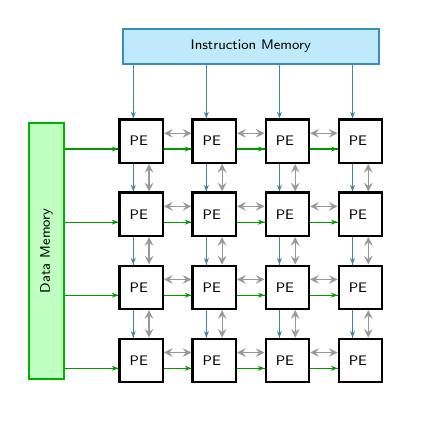
\begin{tikzpicture}[
  pe/.style={
    draw=black, fill=white, thick,
    minimum width=0.55cm, minimum height=0.55cm,
    font=\tiny\sffamily, align=center
  },
  mem/.style={
    draw=#1!70!black, fill=#1!25, thick,
    font=\tiny\sffamily, align=center
  },
  hlink/.style={stealth-stealth, thin, black!40},
  vlink/.style={stealth-stealth, thin, black!40},
  imemlink/.style={-, thin, cyan!60!black},
  dmemlink/.style={-, thin, green!60!black},
  imemtap/.style={-{Stealth[scale=0.5]}, thin, cyan!60!black},
  dmemtap/.style={-{Stealth[scale=0.5]}, thin, green!60!black},
]
  \matrix (grid) [
    matrix of nodes,
    nodes={pe},
    row sep=0.35cm,
    column sep=0.35cm,
  ] {
    |[pe]| PE & |[pe]| PE & |[pe]| PE & |[pe]| PE \\
    |[pe]| PE & |[pe]| PE & |[pe]| PE & |[pe]| PE \\
    |[pe]| PE & |[pe]| PE & |[pe]| PE & |[pe]| PE \\
    |[pe]| PE & |[pe]| PE & |[pe]| PE & |[pe]| PE \\
  };

  \node[mem=cyan,
    minimum width=4*0.55cm + 3*0.35cm,
    minimum height=0.45cm,
    above=0.55cm of grid.north,
    anchor=south,
  ] (IMEM) {Instruction Memory};

  \node[mem=green,
    minimum height=4*0.55cm + 3*0.35cm,
    minimum width=0.45cm,
    left=0.55cm of grid.west,
    anchor=east,
  ] (DMEM) {\rotatebox{90}{Data Memory}};

  \begin{pgfonlayer}{background}
    \foreach \r in {1,...,4} {
      \foreach \c in {1,2,3} {
        \pgfmathtruncatemacro{\cn}{\c+1}
        \draw[hlink] ([yshift=0.10cm]grid-\r-\c.east)
                  -- ([yshift=0.10cm]grid-\r-\cn.west);
      }
    }
    \foreach \c in {1,...,4} {
      \foreach \r in {1,2,3} {
        \pgfmathtruncatemacro{\rn}{\r+1}
        \draw[vlink] ([xshift=0.10cm]grid-\r-\c.south)
                  -- ([xshift=0.10cm]grid-\rn-\c.north);
      }
    }
    \foreach \c in {1,...,4} {
      \draw[imemlink]
        ([xshift=-0.10cm]IMEM.south -| grid-1-\c)
        -- ([xshift=-0.10cm]grid-4-\c.south -| grid-1-\c);
    }
    \foreach \c in {1,...,4} {
      \foreach \r in {1,...,4} {
        \draw[imemtap]
          ([xshift=-0.10cm]grid-\r-\c.north -| grid-\r-\c.center)
          ++(0, 0.10cm)
          -- ([xshift=-0.10cm]grid-\r-\c.north);
      }
    }
    \foreach \r in {1,...,4} {
      \draw[dmemlink]
        ([yshift=-0.10cm]DMEM.east |- grid-\r-1)
        -- ([yshift=-0.10cm]grid-\r-4.east |- grid-\r-1);
    }
    \foreach \r in {1,...,4} {
      \foreach \c in {1,...,4} {
        \draw[dmemtap]
          ([yshift=-0.10cm]grid-\r-\c.west |- grid-\r-\c.center)
          ++(-0.10cm, 0)
          -- ([yshift=-0.10cm]grid-\r-\c.west);
      }
    }
  \end{pgfonlayer}
\end{tikzpicture}
\caption{Targeted $4\times4$ Homogeneous CGRA; 16 PE's with full ALU capability and Memory access, nearest neighbour connection.}
\label{fig:cgra_arch}
\end{center}
\end{figure}

\begin{table}
\centering
\caption{Structural statistics of the training (1500 graphs) and evaluation 
(150 graphs) dataset splits. All values reported as mean $\pm$ std 
(min--max).}
\label{tab:dataset_stats}
\setlength{\tabcolsep}{4pt}
\begin{tabular}{lrr}
\textbf{Metric} & \textbf{Training} & \textbf{Evaluation} \\
\midrule
Nodes           & $22.51 \pm 3.31$ \ (16--28) & $23.16 \pm 2.92$ \ (16--28) \\
Edges           & $21.77 \pm 3.39$ \ (15--29) & $22.45 \pm 2.97$ \ (15--28) \\
Depth           & $8.19 \pm 1.32$ \ (6--13)   & $8.40 \pm 1.30$ \ (6--12)   \\
Parallelism     & $4.26 \pm 0.95$ \ (2--8)    & $4.19 \pm 0.97$ \ (2--7)    \\
Instr-Level Parallelism             & $2.21 \pm 0.45$ \ (1.3--4.0) & $2.21 \pm 0.48$ \ (1.3--3.8) \\
Memory ratio    & $0.42 \pm 0.07$ \ (0.21--0.62) & $0.42 \pm 0.08$ \ (0.25--0.60) \\
\bottomrule
\end{tabular}
\end{table}

To evaluate the performance of the proposed GNN-guided partitioning framework a $4\times4$ homogeneous CGRA was targeted, shown in Fig.~\ref{fig:cgra_arch}. 

A dataset of 1650 DFGs was generated using the synthetic generator described in Section~\ref{subsec:synthetic_dfg_gen}. Of these, 1500 graphs were used to produce ground-truth partition labels for GNN training, and the remaining 150 served as a held-out benchmark set for evaluating five mapping strategies. 

Highly parallelizable graphs impose higher partition counts and routing constraints that are difficult to satisfy under the spatial mapper's nearest-neighbor adjacency requirement (C4). To relax routing pressure and keep training tractable, the training set was biased toward moderately sized, low-to-medium parallelism graphs. \textbf{Table~\ref{tab:dataset_stats}} summarizes the structural statistics of both splits; the two distributions are closely matched, confirming that the evaluation set is representative of the training distribution.

Five partitioning strategies were evaluated to characterize the contribution of each component of the proposed framework. \textsc{SAT-min-k} (Algorithm~\ref{alg:sat-min-k}) serves as the optimal reference, performing an exhaustive search over all valid $K$-partition assignments and returning the minimum-cut solution at the smallest feasible $K$. A greedy list-scheduling partitioner is included as a fast baseline, building partitions in a single irreversible sweep without searching over alternative assignments, representative of conventional compilation heuristics. To isolate the contribution of the guided partitioner independently of the GNN, the topological strategy runs the topology-aware partitioner with no learned input: all nodes are seeded to partition $0$ and boundaries are determined entirely by the convexification and capacity repair steps (Section~\ref{subsec:guided_repair}). The \textsc{GNN-raw} strategy takes per-node partition indices predicted by the GNN and constructs partitions directly from these assignments without any convexification or feasibility repair, submitting them to the SAT-based spatial mapper as-is; this isolates the raw predictive quality of the GNN from the contribution of the repair procedure. Finally, the full \textsc{GNN-guided} strategy seeds the topology-aware partitioner with GNN predictions, combining learned partition structure with topology-aware repair, and constitutes the primary contribution of this work.

The framework operates under two simplifying assumptions. Each partition is assumed to complete execution within a single CGRA configuration cycle, consistent with the one-shot mapping model of the SAT-based spatial mapper and a common assumption in spatial CGRA compilation; it does not account for multi-cycle operations or data-dependent latencies that would require a modulo scheduling pass. Cut edges are materialized as synthetic \textit{store}/\textit{load} pairs at partition boundaries, implying a shared data memory for transferring live values between consecutive configurations. The framework does not model transfer latency or bandwidth, nor architectures using dedicated inter-configuration registers or FIFOs. The number of cut edges serves as a proxy for inter-partition communication overhead under the assumption that each synthetic memory pair incurs a uniform cost.
\clearpage
\subsection{Experimental Results}
% Average edge-cut reduction
% Partition count comparison
% SAT-check reduction
% Results across different CGRA sizes
%
% Example graph visualizations
% Discussion of memory movement implications

\begin{table}[h]
\centering
\caption{Benchmark results on the 150-graph evaluation set. $\dagger$ Greedy results are reported on its 23 successes only and are not directly comparable.}
\label{tab:benchmark_results}
\resizebox{\textwidth}{!}{
\begin{tabular}{lccccc}
& \textsc{SAT-min-k}
& Greedy
& Topological
& \textsc{GNN-raw}
& \textsc{GNN-guided} \\
& \scriptsize{(exhaustive, iterative method)} & \scriptsize{(single-pass, no repair)} & \scriptsize{(topo-aware, unguided)} & \scriptsize{(single-pass, raw GNN predictions)} & \scriptsize{(topo-aware, GNN-guided)} \\
\midrule
Success rate
    & $150/150$\ $(100\%)$
    & $23/150$\ $(15.3\%)$
    & $139/150$\ $(92.7\%)$
    & $106/150$\ $(70.7\%)$
    & $147/150$\ $(98.0\%)$ \\
\midrule
Mean edge cuts
    & $1.31 \pm 0.09$
    & $1.52 \pm 0.37^\dagger$
    & $3.22 \pm 0.25$
    & $1.74 \pm 0.17$
    & $2.15 \pm 0.20$ \\
\midrule
Partitioning (s)
    & $0.581 \pm 0.396$
    & $0.005 \pm 0.001$
    & $0.007 \pm 0.001$
    & $0.0004 \pm 0.00001$
    & $0.004 \pm 0.0004$ \\
SAT mapping (s)
    & $11.508 \pm 2.276$
    & $0.071 \pm 0.004$
    & $0.498 \pm 0.047$
    & $0.071 \pm 0.002$
    & $0.243 \pm 0.039$ \\
SAT checks / partition
    & $80.59 \pm 12.40$
    & $1.00 \pm 0.00$
    & $3.71 \pm 0.21$
    & $1.00 \pm 0.00$
    & $2.36 \pm 0.11$ \\
\bottomrule
\end{tabular}}
\end{table}

\begin{table}[h]
\centering
\caption{Benchmark results restricted to the 106 graphs solved by \textsc{GNN-raw}, i.e.\ the like-for-like subset for the \textsc{GNN-raw} vs.\ \textsc{GNN-guided} comparison. $\dagger$ Greedy results are reported on its 20 successes only and are not directly comparable.}
\label{tab:benchmark_common}
\resizebox{\textwidth}{!}{
\begin{tabular}{lccccc}
& \textsc{SAT-min-k}
& Greedy
& Topological
& \textsc{GNN-raw}
& \textsc{GNN-guided} \\
& \scriptsize{(exhaustive, iterative method)} & \scriptsize{(single-pass, no repair)} & \scriptsize{(topo-aware, unguided)} & \scriptsize{(single-pass, raw GNN predictions)} & \scriptsize{(topo-aware, GNN-guided)} \\
\midrule
Success rate
    & $106/106$\ $(100\%)$
    & $20/106$\ $(18.9\%)$
    & $100/106$\ $(94.3\%)$
    & $106/106$\ $(100\%)$
    & $106/106$\ $(100\%)$ \\
\midrule
Mean edge cuts
    & $1.09 \pm 0.06$
    & $1.55 \pm 0.41^\dagger$
    & $3.00 \pm 0.29$
    & $1.74 \pm 0.17$
    & $1.60 \pm 0.17$ \\
\midrule
Partitioning (s)
    & $0.089 \pm 0.013$
    & $0.005 \pm 0.001$
    & $0.005 \pm 0.0005$
    & $0.0003 \pm 0.00001$
    & $0.002 \pm 0.0001$ \\
SAT mapping (s)
    & $7.923 \pm 1.265$
    & $0.061 \pm 0.004$
    & $0.393 \pm 0.044$
    & $0.060 \pm 0.002$
    & $0.133 \pm 0.028$ \\
SAT checks / partition
    & $70.44 \pm 8.87$
    & $1.00 \pm 0.00$
    & $3.60 \pm 0.24$
    & $1.00 \pm 0.00$
    & $2.01 \pm 0.02$ \\
\bottomrule
\end{tabular}}
\end{table}


% 3 metodos --> iterativos
% gnn guided nao é (+/-)

% topological part + sat mapper

% \paragraph{Feasibility.}
% The greedy strategy succeeds on only $15.3\%$ of graphs, confirming that single-pass list scheduling is not suited for wide, parallel DFGs. Both guided variants achieve high feasibility rates: topological at $92.7\%$ and \textsc{GNN-guided} at $98.0\%$, demonstrating that the repair procedure alone largely solves the feasibility problem independently of the GNN.

% \paragraph{Partition quality.}
% On the common solvable subset, \textsc{SAT-min-k} achieves a mean of $1.31$ edge cuts per graph, establishing the optimality baseline. The topological strategy without GNN guidance produces $3.22$ mean cuts; a gap of $1.91$ cuts above optimal. \textsc{GNN-guided} reduces this to $2.15$ mean cuts, closing approximately $55\%$ of the gap to the \textsc{SAT-min-k} optimum. A similar pattern holds for mean frontier edges, which fall from $3.00$ (topological) to $1.86$ (\textsc{GNN-guided}), approaching the optimal $1.25$.

% The greedy strategy is excluded from this quality comparison: its $15.3\%$ success rate selects only the simplest, most constrained graphs in the evaluation set, so its apparent mean of $1.52$ cuts reflects selection bias rather than partition quality.

% \paragraph{Runtime.}
% \textsc{GNN-guided} (mean $0.20$\,s) is approximately $50\times$ faster than \textsc{SAT-min-k} (mean $9.98$\,s), while producing partitions within $0.84$ cuts of the exact optimum on average. The topological strategy (mean $0.39$\,s) is roughly $2\times$ slower than \textsc{GNN-guided} despite producing worse partitions, because a poor seed requires more feasibility-repair iterations. GNN inference itself contributes approximately $4$\,ms per graph and is negligible relative to the mapping cost.

\paragraph{Feasibility.}
The greedy strategy succeeds on only $15.3\%$ of graphs, confirming that single-pass list scheduling is not suited for wide, parallel DFGs. \textsc{GNN-raw}, which submits raw GNN predictions directly to the SAT mapper without any repair, achieves $70.7\%$, reflecting the current accuracy limitations of the GNN: predictions are occasionally structurally infeasible, but when they are valid they require no repair overhead. Both topology-aware variants achieve high feasibility rates: topological at $92.7\%$ and \textsc{GNN-guided} at $98.0\%$, demonstrating that the repair procedure alone largely solves the feasibility problem independently of the GNN.

\paragraph{Partition quality.}
\textsc{SAT-min-k} (Algorithm~\ref{alg:sat-min-k}) achieves a mean of $1.31$ edge cuts per graph, establishing the optimality baseline. The topological strategy produces $3.22$ mean cuts, a gap of $1.91$ above optimal, which \textsc{GNN-guided} reduces to $2.15$ cuts, closing approximately $55\%$ of the gap. \textsc{GNN-raw} reports $1.74$ mean cuts, but only on the $106$ structurally easier graphs it manages to solve, so this figure is not comparable to the others. Restricting all strategies to those same $106$ graphs (Table~\ref{tab:benchmark_common}) removes the bias: the optimum falls to $1.09$, and \textsc{GNN-guided} ($1.60$ cuts) produces \emph{fewer} cuts than \textsc{GNN-raw} ($1.74$), closing $73\%$ of the gap to the optimum versus $66\%$ for the raw predictions. The repair procedure therefore improves partition quality on top of restoring feasibility, rather than degrading it; the apparent advantage of raw predictions on the full set was an artifact of their restriction to easier graphs.

\paragraph{Runtime.}
\textsc{GNN-raw} is the fastest non-trivial strategy: partitioning takes $0.4$\,ms and SAT mapping $0.07$\,s, matching greedy's per-partition cost since both submit exactly one SAT check per partition. \textsc{GNN-guided} (partitioning $4$\,ms, SAT mapping $0.24$\,s) is approximately $50\times$ faster end-to-end than \textsc{SAT-min-k} (Algorithm~\ref{alg:sat-min-k}) ($12.1$\,s total), while the topological strategy ($0.50$\,s SAT mapping) is slower than \textsc{GNN-guided} despite producing worse partitions, because a poor seed drives more feasibility-repair iterations and consequently more SAT checks per partition ($3.71$ vs.\ $2.36$).

\section{Conclusion}
% Summary of contributions
% Main findings
% Future work:
% - larger CGRAs
% - heterogeneous architectures
% - temporal/modulo scheduling integration

This work presented a GNN-guided partitioning framework for spatial CGRA mapping that learns optimal partition structure from exhaustive SAT-generated ground truth. The proposed flow addresses the case where the DFG does not fit within the CGRA. While most approaches focus on accelerating placement and routing, this work targets the pre-mapping phase.

The framework makes three contributions. First a configurable synthetic DFG generator, which produces training graphs by applying structure-preserving mutations to kernel templates, enabling large-scale dataset generation without relying on compiler-extracted benchmarks. Second an exhaustive \textsc{SAT-min-k} (Algorithm~\ref{alg:sat-min-k}) search provides provably optimal partition assignments as ground-truth labels, ensuring the GNN learns from high-quality supervision. Finally, a topology-aware guided partitioner which translates per-node GNN predictions into feasible partitions through convexification and capacity repair.

Evaluation on a $4 \times 4$ homogeneous CGRA with five strategies shows that the proposed \textsc{GNN-guided} flow is the strongest practical method. On the full evaluation set it achieves a $98\%$ feasibility rate and reduces mean edge cuts by $33\%$ relative to the unguided topological baseline, closing $55\%$ of the gap to the \textsc{SAT-min-k} (Algorithm~\ref{alg:sat-min-k}) optimum at roughly $50\times$ lower runtime. A like-for-like comparison on the $106$ graphs that \textsc{GNN-raw} also solves (Table~\ref{tab:benchmark_common}) clarifies the role of the repair procedure: once graph structure is controlled for, \textsc{GNN-guided} produces fewer cuts than \textsc{GNN-raw} ($1.60$ vs.\ $1.74$, against an optimum of $1.09$), closing $73\%$ of the gap to the optimum versus $66\%$ for the raw predictions. The apparent quality advantage of \textsc{GNN-raw} on the full set was therefore an artifact of its restriction to structurally easier graphs, not evidence that raw seeds are superior; repair both restores feasibility ($98\%$ vs.\ $70.7\%$) and lowers the cut count.

The large gap between the unguided topological baseline ($3.00$ cuts on the common subset) and both GNN-seeded variants confirms that the learned predictions carry strong partition structure, and the residual gap to the optimum reflects prediction error rather than a limitation of the repair mechanism. \textsc{GNN-raw} remains the cheapest option, since it runs one SAT check per partition, but is dominated on both feasibility and cut quality, positioning it as a low-cost fallback rather than the primary method.

Several directions remain open. The current evaluation targets a $4 \times 4$ homogeneous CGRA; scaling to larger grids and heterogeneous architectures, where PEs support different ISA subsets, will stress both the GNN's generalization and the repair procedure's routing assumptions. An alternative GNN formulation predicting cut probability per edge in addition to partition index per node could close the remaining quality gap more directly. Finally, the framework currently assumes single-cycle, one-shot execution per partition; integrating temporal or modulo scheduling would substantially broaden its applicability to real compilation workflows.


\begin{credits}
\subsubsection{\ackname} This work is financed by National Funds through the
FCT -- Fundação para a Ciência e a Tecnologia, I.P.\ (Portuguese Foundation
for Science and Technology) within the project AIMaCoV, with reference 2023.14899.PEX (\url{https://doi.org/10.54499/2023.14899.PEX}).
\end{credits}

\bibliographystyle{splncs04}
\bibliography{refs}
\end{document}
